\documentclass[onecolumn, conference]{IEEEtran}
\IEEEoverridecommandlockouts
% The preceding line is only needed to identify funding in the first footnote. If that is unneeded, please comment it out.

\usepackage{cite}
\usepackage{amsmath,amssymb,amsfonts}
%\usepackage{algorithmic}
\usepackage[ruled]{algorithm2e}
\usepackage{graphicx}
\usepackage{textcomp}
\usepackage{xcolor}
%\usepackage{amsmath}
%\usepackage{ntheorem}
%\usepackage[thmmarks,amsmath]{ntheorem}
\usepackage{bm}
\usepackage{amsthm}
\usepackage[colorlinks,
            linkcolor=red,
            anchorcolor=blue,
            citecolor=blue
            ]{hyperref}
\newtheorem{theorem}{\textbf{Theorem}}
\newtheorem{lemma}{Lemma}
%\newtheorem{proof}{\textit{Proof}}

\def\BibTeX{{\rm B\kern-.05em{\sc i\kern-.025em b}\kern-.08em
    T\kern-.1667em\lower.7ex\hbox{E}\kern-.125emX}}
\begin{document}

\title{ Dominant Invariant Subspace for\\Feature Construction in Reinforcement Learning
}

\author{\IEEEauthorblockN{{\large Tao Huang} \\
Student ID: 2018533172\\
Email: huangtao1@shanghaitech.edu.cn}

\and
\IEEEauthorblockN{{\large Yintian Zhang} \\
Student ID: 2020232168\\
Email: zhangyt@shanghaitech.edu.cn
}
}

\maketitle

\begin{abstract}
	 Generally accompanied with large-scale state spaces, reinforcement learning problems under various backgrounds are naturally addressed through the idea of value function approximation. Linear value function approximation (LVFA), one of the most common and essential approaches, has relatively higher sample efficiency to achieve stable value function and provides advanced insight to nowadays network-based methods. The main challenge of LVFA lies in how to construct reasonable features since prior knowledge about optimal value function is rarely available in practice. Based on the 
	subspace invariance, we propose a new method for feature construction through orthogonal iteration with strongly theoretical guarantees. Moreover, we conduct numerical simulations to verify the empirical outperformance of our method over various baseline algorithms. 
\end{abstract}

\section{Introduction}\label{sec:introduction}

	Recent years have witnessed sensational progress of reinforcement learning (RL) in many challenging sequential decision-making problems, such as playing the game of Go \cite{Mnih2013PlayingAW}\cite{ Silver2017MasteringTG}, robotic control \cite{Lillicrap2016ContinuousCW} and autonomous driving\cite{ShalevShwartz2016SafeMR}. The key idea under RL is modeling the agent to perform sequential decision-making by interacting with environment formulated as a Markov decision process (MDP). 

	In general, RL settings are commonly accompanied with large-scale state spaces, making how to ensure scalability a challenging open problem. Many existing methods based on value function approximation have been proposed to express the value function with some appropriate features \cite{Sutton2005ReinforcementLA, Szepesvari2010AlgorithmsFR, Wang2020OnRR}. Linear value function approximation (LVFA), representing the value function as a linear combination of given features, serves as a common and essential approximation approach among these methods. Specifically, it has relatively higher sample efficiency to  estimate the value function stably due to the simple way of encoding prior knowledge. Moreover, many existing deep RL methods \cite{Mnih2013PlayingAW, Silver2017MasteringTG, Lillicrap2016ContinuousCW, ShalevShwartz2016SafeMR} commonly set a linear output layer where LVFA can be suitably applied to explore insights and interpretability of such network-based methods. 
		
	The key problem in LVFA is how to generate reasonable features that are sufficiently representative to approximate the true value function. This is regraded as a hard task since prior knowledge about true value function is rarely available in practice. Considerable effort has been dedicated to address such a problem in roughly two perspectives. One called  feature selection attempts to select reasonable ones from a set of presented candidate features \cite{Bradtke2004LinearLA, Sutton2005LearningTP, Geramifard2006IncrementalLT, Kolter2009RegularizationAF, Johns2010LinearCF, Petrik2010FeatureSU}. The other known as feature construction, which is the exact focus of this paper, aims to construct representative features automatically without given sets of features\cite{Parr2008AnAO,Petrik2007AnAO ,Parr2007AnalyzingFG,Song2016LinearFE,Behzadian2019FeatureSB}. 
	
	In this work, we propose a method that selects features from the transition matrix and the reward function. Specifically, it adopts orthogonal iteration to find orthonormal features and utilizes subspace invariance to reach great empirical performance with theoretical guarantees. This method is also extended to the case with large-scale state spaces by means of generating features directly from raw input data.

The rest of this paper is organized as follows. In Section~\ref{sec:framework}, we describe the fundamental framework and the notations related to LVFA. Then we  give a brief overview and criticisms of the existing work in Section~\ref{sec:related}. Our contribution including algorithm design and performance analysis is presented in Section~\ref{sec:contribution}, followed by our simulation results and analysis in Section~\ref{sec:simulation}. Finally, Section~\ref{sec:conclusion} concludes this paper with a few remarks on future work.

\section{Framework and Notation}\label{sec:framework}
In this section, we give a brief overview of the fundamental background on linear value function approximation and feature selection in reinforcement learning. Mathematical notations, meanwhile, are introduced for clearer expression throughout this paper. 
\subsection{Markov Decision Process} 
We consider a sequential decision problem formulated as a Markov decision process (MDP) under reinforcement learning settings. Such a process is usually defined by a tuple $\langle \mathcal{S},\mathcal{A},\mathcal{P}, \mathcal{R},\gamma\rangle$, where $\mathcal{S}$ and $\mathcal{A}$ denote the state and action spaces, respectively; $\mathcal{P}: \mathcal{S}\times\mathcal{A} \times \mathcal{S} \rightarrow [0,1] $ denotes the transition probabilities from current state $s\in \mathcal{S}$ to any underlying states $s'\in \mathcal{S}$ given action $a\in \mathcal{A}$; $\mathcal{R}: \mathcal{S}\times\mathcal{A}  \rightarrow \mathbb{R}$ represents the reward function whose element $\mathcal{R}(s,a)$ is the expected instantaneous reward collected by the agent in state $s$ by taking action $a$; $\gamma\in [0,1]$ is the discount factor that determines the present value of future reward.

Based on the aforementioned definitions, we define policy $\pi: \mathcal{S}\rightarrow \mathcal{A}$ as the behavior of the agent in MDPs. Specifically, at each time slot $t$, $a_t\sim \pi(\cdot|s_t)$ denotes a mapping from state $s_t$ to the distribution over the whole action space $\mathcal{A}$. It basically characterizes the agent's way of decision-making under given state $s\in \mathcal{S}$. Accordingly, we define value function $v_\pi(s)$ as the expected discounted cumulative reward (return) starting from state $s\in\mathcal{S}$, which can be expressed as
	\begin{equation}
		v_\pi (s) = \mathbb{E}\left[\sum_{t\ge 0}\gamma^{t} \mathcal{R}(s_t,a_t)\Big| a_t \sim \pi(\cdot|s_t),s_0=s \right].
	\end{equation}
By denoting $\boldsymbol{v}^{\pi}$ as the state-values in a vector form under a given policy $\pi$, we have the following Bellman equation \cite{Puterman1994MarkovDP}:
	\begin{equation}\label{Bellman Equation}
		\boldsymbol{v}^\pi = \boldsymbol{r}^\pi +\gamma P^\pi \boldsymbol{v}^\pi,
	\end{equation}
	where $P^\pi$ and $\boldsymbol{r}^\pi$ are the transition probability in a matrix form and rewards in a vector form under policy $\pi$, respectively. 
\subsection{Linear Value Function Approximation}\label{subsec: LVFA}
 Linear value function approximation plays a key role in solving MDPs, especially with large-scale state spaces $\mathcal{S}$. It characterizes the value function in a parametric way, approximating the value of states as the linear combination of a set of $k$ linear independent features $\Phi = \{\phi_1,..., \phi_k\}$:
 	\begin{equation}
 		\hat{\boldsymbol{v}}^{\pi} =  \Phi \boldsymbol{w},
 	\end{equation}
 	where $\phi_i \in \mathbb{R}^{|\mathcal{S}|}$ denotes the feature vector over state space $\mathcal{S}$ and $\boldsymbol{w} \in \mathbb{R}^k$ is the weight vector of the features. The task is how to find an appropriate weight vector $\boldsymbol{w}$ to approximate the true value function accurately.
 	
\subsubsection{Fixed-Point Method} Methods in \cite{Bradtke2004LinearLA, Sutton2005LearningTP, Geramifard2006IncrementalLT} have been proposed to estimate a reasonable weight vector $\boldsymbol{w}$ given the features $\Phi$. It is further proved in \cite{Koller1999ComputingFV} that there exists unique weight vector $\boldsymbol{w}^\pi_\Phi$ which can be found by linear \textit{fixed-point method}:
	\begin{equation}\label{fixed-point method}
		\hat{\boldsymbol{v}}^{\pi} = \Phi \boldsymbol{w}_\Phi^\pi  = \Pi_\sigma (\boldsymbol{r}^\pi + \gamma P^\pi \Phi \boldsymbol{w}_\Phi^\pi ).
	\end{equation}
	where $\Pi_\sigma$ represents the the $\sigma$-weighted $L_2$ projection into $span(\Phi)$ and $\sigma$ is a state weighting distribution, which is reasonably assumed unweighted in this paper due to the independence with projection weights. It can be solved by least square approach or by applying orthogonal projector to both sides of \eqref{Bellman Equation}. Both of them give the $\boldsymbol{w}^\pi_\Phi$ as:
	\begin{equation}\label{fixed-point solution}
		\begin{split}
		\boldsymbol{w}_\Phi^\pi &= \Phi^{\dagger} (\boldsymbol{r}^\pi + \gamma P^\pi \Phi \boldsymbol{w}_\Phi^\pi )\\
		&= (I-\gamma \Phi^{\dagger} P^\pi \Phi )^{-1}\Phi^{\dagger}\boldsymbol{r}^\pi,
		\end{split}
	\end{equation}
	where $\Phi^{\dagger} = (\Phi^T\Phi)^{-1}\Phi^T$ is the Moore-Penrose pseudo-inverse of the features $\Phi$ \cite{EtAl2007MatrixC3}. The results have been extended to Q-functions in \cite{Song2016LinearFE} with theoretical guarantees.
\subsubsection{Linear Model} Another approach of desired unique weight vector $\boldsymbol{w}$ is by constructing a linear model in which the transition matrix $P^{\pi}$ and rewards $\boldsymbol{r}^\pi$ are compressed as $P^{\pi}_\Phi \in \mathbb{R}^{k\times k}$ and $\boldsymbol{r}^{\pi}_\Phi\in \mathbb{R}^{k}$:
	\begin{equation}\label{compress P}
		P^{\pi}_\Phi = \Phi^{\dagger}P^\pi\Phi, \quad \boldsymbol{r}^{\pi}_\Phi = \Phi^{\dagger}\boldsymbol{r}^{\pi}.
	\end{equation}
	The above expressions follow from solving the least-square problem with the goal aiming to predict the next expected feature values and rewards, respectively. It has been proved that the solution of such a model is equivalent to which in \eqref{fixed-point solution} \cite{Parr2008AnAO}. Specifically, the solution yields by solving the “compressed" Bellman equation:
	\begin{equation}
		\begin{split}
			\boldsymbol{w}_\Phi^\pi &= \boldsymbol{r}_\Phi^\pi + \gamma P_{\Phi}^{\pi}\boldsymbol{w}_\Phi^\pi\\
			&=(I - \gamma P_{\Phi}^{\pi})^{-1} \boldsymbol{r}_\Phi^\pi,
		\end{split}
	\end{equation} 
	which can be simplified as the form in \eqref{fixed-point solution} by substituting for $P_{\Phi}^{\pi}$ and $\boldsymbol{r}_\Phi^\pi$.
\subsubsection{Bellman Operator and  Bellman Error} To simplify the notion for operating value function, we hereby define the Bellman operator $T^\pi$ on the value function $\boldsymbol{v}$ as 
        \begin{align}
            T^\pi\boldsymbol{v} = \boldsymbol{r}^\pi +\gamma P^\pi \boldsymbol{v}.
        \end{align}
		$\boldsymbol{v}^\pi$ is known as a fixed point of $T^\pi$, \textit{i.e.} $T^\pi \boldsymbol{v}^\pi = \boldsymbol{v}^\pi$. Note that defining $ \boldsymbol{v}^0 = \boldsymbol{r^\pi}$, then $\boldsymbol{v}^{t+1} = (T^\pi)^t \boldsymbol{r}^\pi$, results in the value iteration algorithm where $\boldsymbol{v}^t \rightarrow \boldsymbol{v}^\pi$ as $t$ increases. We will see that this property is naturally adopted to construct features in \ref{subsec:overview}. The Bellman error/residual is introduced to analyze the error under the value function $\boldsymbol{v}^{\pi}$ given the transition matrix $P^{\pi}$ and rewards $\boldsymbol{r}^{\pi}$ \cite{Williams1993TightPB}, which is defined as
		\begin{align}
		    BE(\boldsymbol{v}) = T^\pi \boldsymbol{v}  - \boldsymbol{v}.
		\end{align}
		When the Bellman error is 0, the value function $\boldsymbol{v}$ is at the fixed point. Otherwise, the distance between $\boldsymbol{v}$ and $\boldsymbol{v}^\pi$ is bounded in terms of the Bellman error:
		\begin{align}\label{equation:VBE}
			\Vert \boldsymbol{v} - \boldsymbol{v}^\pi \Vert_{\infty} 
			\le  \Vert \boldsymbol{v} - T^\pi \boldsymbol{v}\Vert_{\infty} + \Vert T^\pi\boldsymbol{v} - \boldsymbol{v}^\pi \Vert_{\infty} 
			\le BE(\boldsymbol{v} ) + \gamma \Vert \boldsymbol{v} -  \boldsymbol{v}^\pi\Vert_{\infty}  
			\le \frac{BE(\boldsymbol{v})}{1-\gamma}.
		\end{align}
		where $\Vert \boldsymbol{v} \Vert$ refers to the $\ell_\infty$ norm of a vector $\boldsymbol{v}$.
		
		 In the context of linear value function approximation, such a metric is naturally extended to quantify the quality of the selected features. Specifically, the Bellman error is redefined as the error in the linear fixed-point value function $\boldsymbol{v}_\Phi^\pi$ for given features $\Phi$:
	\begin{equation}
		\begin{split}
			BE(\Phi) & = T^\pi (\Phi \boldsymbol{w}_\Phi^\pi) - \Phi \boldsymbol{w}_\Phi^\pi\\
			&= \boldsymbol{r}^\pi + \gamma P^\pi \Phi \boldsymbol{w}_\Phi^\pi - \Phi \boldsymbol{w}_\Phi^\pi .
		\end{split}
	\end{equation}
The following theorem specifies that Bellman error can be decomposed into two separate sources of error.
\begin{theorem}\label{decomposition}
		For any MDP with given feature $\Phi$ and policy $\pi$, the Bellman error of a value function $\hat{\boldsymbol{v}}^\pi=\Phi \boldsymbol{w}_\Phi^\pi$ can be decomposed as\cite{Parr2008AnAO}:
		\begin{equation}
		\begin{split}
			BE(\Phi) &=   \underbrace{(\boldsymbol{r}^\pi - \Phi \boldsymbol{r}_\Phi^\pi)}_{\Delta_R^{\pi}} + \gamma \underbrace{(P^\pi \Phi - \Phi P_\Phi^\pi)}_{\Delta_\Phi^\pi}\boldsymbol{w}_\Phi^{\pi}\\ &\triangleq \Delta_R^{\pi} +\gamma \Delta_\Phi^\pi \boldsymbol{w}_\Phi^{\pi},
		\end{split}
		\end{equation}
where $\Delta_R^{\pi}$ and $\Delta_\Phi^\pi$ corresponds to \textit{reward error} and \textit{per-feature error}, respectively. 
	\end{theorem}
	In the next sections, we will show that such a decomposition can guide the process of generating features.
\section{Related Work}\label{sec:related}
There has been great interest in recent years in feature selection and automating feature construction for reinforcement learning. The main difference between these two approaches is that feature selection assumes a reasonable set of candidate features are presented to the learner, while such a presumably given set is rarely available in feature-construction's view. 

Accordingly, for the former, the task is to select a small set of features to prevent over-fitting and expensive computational cost. This is difficult and requires a deep understanding of the domain. For the latter, the focus is how to automatically construct features representative enough to approximate the real value function. Meanwhile, priority should be given to scalability to ensure practical feasibility. In the remainder of this section, we give a brief overview of the existing work in the perspective of the two aforementioned approaches, followed by the criticisms of these work.
\subsection{Overview of the Existing Work}\label{subsec:overview}
\subsubsection{Feature Selection}\label{} For the task of linear value function approximation, Least-Squares Temporal Difference (LSTD) algorithms \cite{Bradtke2004LinearLA, Sutton2005LearningTP, Geramifard2006IncrementalLT} provide a basic approach for learning the value function using only trajectories generated by the system. However, these methods are prone to over-fitting and are computationally expensive, especially when the number of features is large compared to the number of training samples. 

To overcome such a challenge, Kolter et al.\cite{Kolter2009RegularizationAF} proposed a regularization framework as LARS-TD for linear value function approximation within LSTD. It employs the technique of regularization to find the sparse solution and therefore serves as an effective method for feature selection:
\begin{align*}
    \boldsymbol{w}_\Phi^\pi &= (\Phi^T\Phi + \beta I)^{-1}\Phi^T(\boldsymbol{r}^\pi + \gamma P^\pi\Phi \boldsymbol{w}_\Phi^\pi)\\
    &=\left(\Phi^T(\Phi - \gamma P^\pi\Phi)+\beta I \right)^{-1} \Phi^\pi \boldsymbol{r}^\pi,
\end{align*}
where $\beta \in [0,\infty)$ is a $l_1$ regularization parameter. 

Johns et al.\cite{Johns2010LinearCF} formulated the $L_1$ regularized linear fixed point problem (Subsection~\ref{subsec: LVFA}) as a linear complementarity problem (LCP):
\begin{align*}
    A^{-1} = \Phi^T(\Phi-\gamma P^\pi\Phi)&,\quad b = \Phi^T\boldsymbol{r}^\pi,\quad c = b-A\boldsymbol{w}\\
    \boldsymbol{w} = A^{-1}b &+ A^{-1}(-c).
\end{align*}
It allows the appropriate utilization of the rich theory of LCPs and provides strong theoretical guarantees with fast performance. Besides, policy iteration method is found more effective through this approach than previous methods.

Petrik et al.\cite{Petrik2010FeatureSU} considered feature selection as an optimization problem with particular $L_1$ regularization (RALP). Specifically, they integrated the approximate linear programming (ALP) with $L_1$ regularization to automate feature selection and alleviate the need for all constraints in standard ALP:
\begin{equation*}
\begin{aligned}
&\min_{\boldsymbol{w}} \quad \boldsymbol{\rho}^T\Phi\boldsymbol{w}\\
&\begin{array}{r@{\quad}r@{}r@{\quad}r}
s.t. &T^\pi (\Phi\boldsymbol{w})\le \Phi \boldsymbol{w} \quad \Vert\boldsymbol{w}\Vert_{1} \le \psi,
\end{array}
\end{aligned}
\end{equation*}
where $\boldsymbol{\rho}$ is a distribution over the initial states (\textit{i.e.,} $\sum_{s\in \mathcal{S}} \rho(s)=1$), and $\Vert\boldsymbol{w}\Vert_{1}\le \psi$ is $L_1$ constraint. Their method offers some strong guarantees, but is not well-suited to noisy sampled data. 

\subsubsection{Feature Construction}\label{subsub:FC}To understand the relationship between the error in the linear model and the Bellman error, Parr et al. \cite{Parr2008AnAO} proved that Bellman error can be decomposed into two separate source of error (Theorem~\ref{decomposition}),
		\begin{equation*}
		\begin{split}
			BE(\Phi) &=   \underbrace{(\boldsymbol{r}^\pi - \Phi \boldsymbol{r}_\Phi^\pi)}_{\Delta_R^{\pi}} + \gamma \underbrace{(P^\pi \Phi - \Phi P_\Phi^\pi)}_{\Delta_\Phi^\pi}\boldsymbol{w}_\Phi^{\pi}
		\end{split}
		\end{equation*}
Recall that $\Delta_R^{\pi}$ and $\Delta_\Phi^\pi$ corresponds to \textit{reward error} and \textit{per-feature error}, respectively. It provides a theoretical framework for constructing the basis feature functions, giving insights into the behavior of existing feature-construction algorithms.

Petrik et al. \cite{Petrik2007AnAO} proposed a method aiming to achieve no reward error. They build a Krylov basis \cite{EtAl2007MatrixC3} in terms of powers of transition matrix $P$ multiplied by reward $\boldsymbol{r}$ as the features:
\begin{align*}
    \Phi^K_k = Krylov_k(\boldsymbol{r}) = \{P^{i-1}\boldsymbol{r}:1\le i \le k\}.
\end{align*}
As the true value function is conceptually defined as $\boldsymbol{v}^\pi = \sum_{t=1}^\infty \gamma^{t}(P^{\pi})^t\boldsymbol{r^\pi}$, their method is regarded as an intuitive design for value iteration, where the value functions of all iterations can be exactly represented by such a Krylov basis $\Phi_k^K$.

Parr et al. \cite{Parr2007AnalyzingFG} modeled the problem of constructing features as basis expansion. That is, given a set of basis functions (features) $\Phi_k^B = \{\phi_1,...,\phi_k\}$ and the a linear fixed point solution, what is a good $\phi_{k+1}$ to extend the basis? They addressed this sequential problem by generating the next feature as the Bellman error $BE(\Phi_k^B)$ of the current fixed point solution $\boldsymbol{v}_{\Phi_k}^\pi$,
	\begin{align*}
		\phi_{k+1} = T^\pi \boldsymbol{v}_{\Phi_k}^\pi - \boldsymbol{v}_{\Phi_k}^\pi = BE(\Phi_k), \quad \Phi_{k+1} = \{\Phi_k^B, \phi_{k+1}\},
	\end{align*}
where $\phi_{k+1}$ is called as Bellman error basis functions. Parr et al. \cite{Parr2008AnAO} have shown that Krylov bases and BEBF span the same approximation space $ span\{\Phi^K_k\}=span\{\Phi_k^B\}$. 

Song et al. \cite{Song2016LinearFE} developed a theory of linear value function encoding. Inspired by the decomposition of Bellman error (Theorem~\ref{decomposition}), they aim to encode a reduced features that are representative enough to approximate the next expected raw features $P^\pi A$ and next reward $\boldsymbol{r}^\pi$. In order to determine the reasonable structure of encoder and decoder, they define \textit{predictively optimal set} of features as follows:
	\begin{align*}
		AE_\pi D_\pi = [P^\pi A, \boldsymbol{r}^\pi]
	\end{align*}
where $D_\pi$ and $E_\pi$ are encoder and decoder, respectively. They have proved that the Bellman error is zero if such a tuple $\langle A,E_\pi,D_\pi \rangle$ can be found. Therefore, the proposed algorithm linear feature discovery (LFD) attempts to minimize the distance from $AE_\pi D_\pi$ to $[P^\pi A, \boldsymbol{r}^\pi]$ based on gradient descent method.

Behzadian et al. \cite{Behzadian2019FeatureSB} utilized the low-rank factorization to construct features directly from raw features, specifically applying singular value decomposition to the compressed transition matrix $P^\pi$ and including reward as one of the features as well. Their method (SVD+R) is proved as efficient method in both small-scale case and large-scale case with bounded theoretical Bellman error. The main difference between SVD+R and LFD is that the former attempts to reduce the raw features through encoder, while the latter dedicates to predict the next expected raw features through low-dimension representations directly.
\subsection{Criticism of the Existing Work}\label{subsec:criticism}
LSTD-based algorithms \cite{Bradtke2004LinearLA, Sutton2005LearningTP, Geramifard2006IncrementalLT} built a basic approach for approximation value function under LVFA's settings. But these methods do not consider the scale of features, leading to the failure of handling the over-fitting and expensively computational cost. To deal with such a challenge, Kolter et al.\cite{Kolter2009RegularizationAF} proposed a regularization framework as LARS-TD for LVFA within LSTD. However, this method is not well-integrated with least squares policy iteration (LSPI) \cite{Lagoudakis2003LeastSquaresPI} algorithm due to the  hardly any exploitation of previous fixed point solution. Based on the LCP, Johns et al.\cite{Johns2010LinearCF} proposed an algorithm that is well-employed by policy iteration. Nonetheless, the incorporation between policy improvement and LCP is considerably inflexible so that practical feasibility comes as a new challenge. Petrik et al.\cite{Petrik2010FeatureSU} considered feature selection from the view of optimization with particular $L_1$ regularization. But their analysis does not address the conditions that would guarantee sparse RALP solutions and it is not well-suited to noisy, sampled data.
    
Recall that feature selection assumes that reasonable features are available to learners. Therefore, in practice, these methods \cite{Bradtke2004LinearLA, Sutton2005LearningTP, Geramifard2006IncrementalLT, Kolter2009RegularizationAF, Johns2010LinearCF, Petrik2010FeatureSU} do not address the problem of how to generate representative features in the first place. This naturally leads to the researches of feature construction which is considered a more basic problem. 

Parr et al. \cite{Parr2008AnAO} proved that Bellman error can be decomposed into two separate sources of error. But their theoretical results are not extended to the controlled case. Specifically, they did not provide the connection between model 
error given a set of features and Bellman error of a Q-function based on these features. Petrik et al. \cite{Petrik2007AnAO} proposed a method BEBF of great intuition, aiming to eliminate the reward error. However, the transition matrix must be approximated in a tabular manner and the resulting basis ${\Phi_k^K}$ is not orthonormal, incurring the high computational expense. Parr et al. \cite{Parr2007AnalyzingFG} proposed using Bellman error to guide the sequential construction of features. But this method is not scalable since both large-scale state spaces and large number of features 
contribute to the time consumption.
Song et al. \cite{Song2016LinearFE} extended the connection between model error and Bellman error to the controlled case and developed linear feature encoding theory for LVFA. However, their method exists two main limits. On one hand, the proposed predictively optimal tuple $\langle A,E_\pi,D_\pi\rangle$~(\ref{subsub:FC}) is almost impossible to be found in practice. On the other, the utilization of iterative learning strategy introduces an additional Bellman error, while theoretical analysis are not clear in this case. Behzadian et al. \cite{Behzadian2019FeatureSB} applied singular value decomposition to approximate the transition matrix $P^\pi$. Nonetheless, the assumption about the low-rank transition matrix is deemed unreasonable, since such low-rank matrices are rare in practice. Therefore, the bound of Bellman error is theoretically loose and empirically large, leading to the mediocre performance in experiments.
\section{New contribution}\label{sec:contribution}


Our method is highly related to the algorithm in \cite{Song2016LinearFE}\cite{Behzadian2019FeatureSB}. The impovements mainly lies in the point that, with milder assumption and great scalability, our algorithm theoretically achieves a tighter Bellman error bound and empirically reaches better performance. 

In the remainder of this section, we give specific illustration of the proposed method DISCO for constructing features from transition matrix and rewards. First, we describe the method assuming that it is possible to represent the value function in a tabular form. Subsequently, we present a extended version of this method to fit the infinite state spaces to ensure scalability, treating raw feature inputs (such as images) as intermediate simplifying features.
\vspace{4pt}

\begin{algorithm}[H]
% \SetAlgoNoLine  %去掉之前的竖线
        \caption{Orthogonal Iteration}\label{OI}
        \KwIn{${\bf A} \in \mathbb{C}^{n\times n}$ and desired number of output vectors $k$.}


        Initialization: $j = 0$, semi-unitary matrix ${\bf V}^{(0)}\in \mathbb{C}^{n\times k}$; \\
        \Repeat{a stopping rule is satisfied}{        	$\tilde{{\bf V}}^{(j+1)} = {\bf A}{\bf V}^{(j)}$\;
        	${\bf V}^{(j+1)} {\bf R}^{(j+1)} = \tilde{{\bf V}}^{(j+1)}${\color{blue}\tcc*{ normalization; perform thin QR for $\tilde{{\bf V}}^{(j+1)}$}}
        	$\{\lambda_1^{(j+1)}, \lambda_2^{(j+1)}, \dots,\lambda_r^{(j+1)}\} = \sigma\left( ({\bf V}^{(j+1)})^H{\bf A}{\bf V}^{(j+1)}  \right)$\;
        	$j := j+1$\;
        	}
             \KwOut{${\bf V}^{(j)}$.}
\end{algorithm}
\subsection{DISCO for Finite State Space}\label{sec:small scale}

Our algorithm design is essentially guided by the Theorem~\ref{decomposition}, where the key idea is to minimize the per-feature error $\Delta_\Phi^\pi$ and reward error $\Delta_R^{\pi}$ separately. For the former, we eliminate such an error $\Vert P^\pi \Phi - \Phi P^\pi_\Phi\Vert_2$ by utilizing subspace invariance defined as $P^\pi\Phi \in span\{\Phi\}$. In particular, we apply orthogonal iteration to construct orthonormal features for the dominant invariant subspace of transition matrix $P^\pi$. For the latter, we achieve zero error by the means of including rewards $\boldsymbol{r}^\pi$ in the features. The intuition comes directly from the properties of orthogonal projection that $\boldsymbol{r}^\pi$ itself is in the range space of $\Phi$.

\vspace{4pt}
\begin{algorithm}[H]
% \SetAlgoNoLine  %去掉之前的竖线
        \caption{DISCO: Dominant Invariant Subspace for Feature Construction\label{EVD+R1}}
        \KwIn{Transition matrix $P^\pi$, rewards $\boldsymbol{r}^\pi$, and number of features $k$.}
        Compute orthogonal Iteration: ${\bf V} = Algorithm~{\ref{OI}}\left(P^\pi, k\right)$\;
        Approximate features: $\Phi = [{\bf V}, \boldsymbol{r}^\pi ]$\;
        \KwOut{$\Phi$.}
\end{algorithm}
\vspace{4pt}
Note that the existence of eigendecomposition is not a necessary condition here, since we only require a few basis vectors of dominant invariant subspace as features to approximate the value function. This attractive property ensures both low computational expense and practical feasibility. The following theorem specifies that the separate design of our algorithm implies a zero Bellman error. 
\pagebreak
\begin{theorem}\label{theorem:tabular}
Given featrues $\Phi$ output from Algorithm \ref{EVD+R1}, the Bellman error $BE(\Phi)=0$ under policy $\pi$. 
\end{theorem}
\begin{proof}
Substitute $\Phi$ into the definition of compressed transition matrix $P_\Phi^\pi$~\eqref{compress P}:
\begin{align*}
    P_\Phi^\pi &= \Phi^\dagger P^\pi\Phi\\
    &= (\Phi^T\Phi)^{-1}\Phi^T P^\pi\Phi\\
    &= \Phi^T P^\pi\Phi\\
    &=\Phi^T \Phi \Lambda\\
    &= \Lambda,
\end{align*}
where the third and the fifth equality comes from the fact that the output basis are orthonormal (ensured by normalized QR), and the forth equality follows from the subspace invariance $P^\pi \Phi = \Phi\Lambda$. Substituting it into the expression of per-feature error $\Delta_\Phi^\pi$~(Theorem \ref{decomposition}), we get:
\begin{align*}
    \Vert \Delta_\Phi^\pi \Vert_2 &= \Vert P^\pi \Phi - \Phi P_\Phi^\pi \Vert_2\\
    &= \Vert \Phi \Lambda - \Phi \Lambda \Vert_2\\
    &= 0,
\end{align*}
where the second equality follows from the subspace invariance. Then we derive the bound of reward error: 
\begin{align*}
	\Vert\Delta_R^\Phi \Vert_2 & = \Vert \boldsymbol{r}^\pi -\Phi\Phi^\dagger \boldsymbol{r}^\pi \Vert_2\\
	& = \Vert \boldsymbol{r}^\pi - \Phi(\Phi^T\Phi)^{-1}\Phi^T \boldsymbol{r}^\pi \Vert_2\\
	&=  \Vert \boldsymbol{r}^\pi - \Phi\Phi^T \boldsymbol{r}^\pi \Vert_2\\
	&=0,
\end{align*}
where the last equality follows directly from the properties of orthogonal projection since $\boldsymbol{r}^\pi$ itself is in the range space of $\Phi$. By applying triangular inequality and Cauchy Schwarz's inequality, we directly derive the Bellman error bound:
\begin{align*}
    \Vert BE(\Phi)\Vert_2 &= \Vert \Delta_R^{\pi} +\gamma \Delta_\Phi^\pi \boldsymbol{w}_\Phi^{\pi}\Vert_2\\
    &\le \Vert \Delta_R^{\pi}\Vert_2 + \gamma\Vert \Delta_\Phi^\pi\Vert_2 \Vert \boldsymbol{w}_\Phi^\pi\Vert_2\\
    &=0,
\end{align*}
which implies Bellman error $BE(\Phi) =0$ due to the non-negativity of norm. 
\end{proof}
For most RL problem, the scale of the state space is almost infinite so that the transition matrix and reward vector used in Algorithm \ref{EVD+R1} will be too large to work with. To make our method more practical, we present an extended version of DISCO in the next subsection.
\subsection{DISCO for Infinite State Space}
\label{sec:big scale}
Inspired by the approaches proposed by \cite{Song2016LinearFE}\cite{Behzadian2019FeatureSB}, we first use a source of raw features, such as the image in video games, to compress the matrix of transition probability matrix. Then we conduct Algorithm \ref{EVD+R1} on these compressed transition matrix and reward vector, followed by the multiplication with raw feature, to reduce the dimension of representations. We give mathematical descriptions in the following part for clearer expression. 

Let $A$ be an $|S| \times l$ matrix, where each row corresponds to a state and each column corresponds to one raw feature, such as the grey value of a pixel. The compressed transition matrix $P^{\pi}_{A}$ and the compressed rewards $\boldsymbol{r}_A$ are defined as 
\begin{align*}
		P^{\pi}_A = A^{\dagger}P^\pi A \triangleq A^{\dagger} A' ,\quad\quad \boldsymbol{r}^{\pi}_A = A^{\dagger}\boldsymbol{r}^{\pi},
\end{align*}
where $A'$ denotes the expected next raw features. The dimensions of  $P^{\pi}_{A}$ and  $\boldsymbol{r}^{\pi}_A$ are now corresponding to the number of raw features. Once they are estimated, we conduct DISCO algorithm \ref{EVD+R1} with them instead of  $P^{\pi}$ and $\boldsymbol{r}^{\pi}$ to get the encoded features $\Phi_{E}$, which is of a dimension $l \times k$. Finally, we construct the ultimate features $\Phi_D$ by multiplying with $A$. We show the pseudo code of such process in Algorithm~\ref{theorem:nontabular}.  

\begin{algorithm}[H]
% \SetAlgoNoLine  %去掉之前的竖线
        \caption{DISCO for Infinite State Space}\label{EVD+R2}
        \KwIn{Raw features $A$, expected next raw features $A'$, rewards $\boldsymbol{r}^\pi$, and number of features $k $.}
        Compute compressed transition matrix: $P^{\pi}_A = A^\dagger A'$\;
        Compute compressed reward: $\boldsymbol{r}^{\pi}_A = A^\dagger \boldsymbol{r}^\pi$\;
        Encoded features: $\Phi_E = Algorithm~\ref{EVD+R1}\left(P^{\pi}_A, \boldsymbol{r}^{\pi}_A, k \right)${\color{blue} \tcc*{Encode raw features $A$ into $\Phi_E$}}
        Decoded features: $\Phi_D = A\Phi_E${\color{blue}\tcc*{Decode $\Phi_E$  into a reduced size features $\Phi_D$}}
        \KwOut{$\Phi_D$.}
\end{algorithm}

This algorithm allows the subsequent operations on the encoded features $\Phi_E$ rather than raw features to lower the computational expense. Simple and practical as it is, we still catch that the final features $\Phi_D$ is a linear combination of the raw features, implying they cannot express more complex value functions. This is intuitively reasonable in the view of bias-variance tradeoff, where additional error is introduced—akin to bias—but sampling error is reduced—akin to variance. The following theorem gives the bound of new-introduced error and how it affect the Bellman error with respect to features $\Phi_D$.
\begin{theorem}\label{theorem:nontabular}
	Assume that the raw features $A$ and encoded features $\Phi_E$ are normalized, \textit{i.e.,} $\Vert A\Vert_2 = \Vert \Phi_D\Vert_2 = 1$. Then:
		\begin{align*}
			\Vert \Delta_{P}^{\Phi_D}\Vert_2 \le \Vert \Delta_P^A\Vert_2 + \Vert \Lambda-P_{\Phi_D} \Vert_2,\quad \Vert\Delta_R^{\Phi_D}\Vert_2 \le \Vert \Delta_R^{A}\Vert_2 + \Vert \Delta_{R_A}^{\Phi_E} \Vert_2 
		\end{align*} 
		where the superscript and subscript of $\Delta$ represents the features and the model (\textit{i.e.,} $\Delta_P^A = PA - AP_A$), respectively. Here we omit the the policy $\pi$ in superscripts for simplicity.
\end{theorem}
\begin{proof}
	 By adding a zero item $(AP_A\Phi_E - AP_A\Phi_E)$ and applying triangular inequality and Cauchy Schwarz's inequality, we get:
	 \begin{align*}
	 	\Vert \Delta_P^{\Phi_D}\Vert_2 & = \Vert P\Phi_D - \Phi_DP_{\Phi_D}\Vert_2\\
	 	& =  \Vert P\Phi_D - AP_A\Phi_E + AP_A\Phi_E - \Phi_DP_{\Phi_D}\Vert_2 \\
	 	& \le \Vert  PA\Phi_E - AP_A\Phi_E\Vert_2 + \Vert AP_A\Phi_E - A\Phi_E P_{\Phi_D}\Vert_2\\
	 	& \le \Vert PA -AP_A\Vert_2 + \Vert \Phi_E \Lambda - \Phi_E P_{\Phi_D}\Vert_2 \Vert A\Vert_2\\
	 	& \le  \Vert \Delta_P^A\Vert_2 + \Vert \Lambda - P_{\Phi_D}\Vert_2\\
	 \end{align*}
	 Similarly, we derive the bound of reward error as:
	 \begin{align*}
	 	\Vert \Delta_R^{\Phi_D}\Vert_2 &= \Vert \boldsymbol{r} - A\boldsymbol{r}_A +A\boldsymbol{r}_A - \Phi_D \boldsymbol{r}_{\Phi_D} \Vert_2\\
	 	&\le \Vert \boldsymbol{r} - A\boldsymbol{r}_A \Vert_2+\Vert A\boldsymbol{r}_A - A\Phi_E \boldsymbol{r}_{\Phi_D} \Vert_2\\
	 	&\le \Vert \boldsymbol{r} - A\boldsymbol{r}_A \Vert_2 + \Vert \boldsymbol{r}_A - \Phi_E \boldsymbol{r}_{\Phi_D} \Vert_2 \\
	 	& = \Vert \Delta_R^{A}\Vert_2 + \Vert \Delta_{R_A}^{\Phi_E} \Vert_2
	 \end{align*}
	 Note that the normalization of raw features $A$ in Theorem \ref{theorem:nontabular} has no effect on approximating the value function, since the the linear fixed point is invariant with such operation. However, it does change the scale of weight vector $\boldsymbol{w}_\Phi$.
\end{proof}

\subsection{Relationship to LFD and SVD+R}
Both DISCO and LFD in \cite{Song2016LinearFE} apply the idea of reducing the representations' dimension for greater scalability. But the main difference between these two algorithms is that the former attempts to reduce the raw features through an encoder, while the latter dedicates to predict the next expected raw features through low-dimension representations directly. We consider ours a more practical method due to two aspects. On one hand, the proposed predictively optimal tuple $\langle A,E_\pi,D_\pi\rangle$~(\ref{subsub:FC}) is almost impossible to be found in practice. On the other, the utilization of iterative learning strategy introduces an additional Bellman error and time consumption, and theoretical analysis are not clear in this case. 

As for DISCO and SVD+R proposed in\cite{Behzadian2019FeatureSB}, they both construct ultimate features by the multiplication with raw features. Nonetheless, the assumption about the low-rank transition matrix in SVD+R is deemed unreasonable, since such low-rank matrices are rare in practice. Rather, this assumption is not necessary in DISCO. The bound of Bellman error in SVD+R, therefore, is theoretically loose and empirically large, leading to the mediocre performance in experiments comparing to DISCO.


\section{Numerical results}\label{sec:simulation}
In this section, we empirically compare some methods that we have discussed in previous sections. Here we use an image-based version of the Cart-Pole benchmark to compare the solution quality of DISCO, SVD+R and LFD algorithms. In the following subsections, we first introduce the basic settings of Cart-Pole. Simulation results are presented next, followed by our evaluation and analysis.
\subsection{Cart-Pole}
The Cart-Pole environment is a complex reinforcement learning benchmark problem. The controller should push the cart left or right to 
ensure the pole on the top of the cart stay vertical as long as possible. The measurement of the performance of the controller is 
the balanced steps in each episode. 
And in our experiment, the controller must learn a policy by merely observing the \textit{image} of the Cart-Pole game 
screen without direct access to the position of the cart or the angle of the pole. 

To obtain training data, we collected the specified number of trajectories with the starting angle and angular velocity 
sampled uniformly on $[-0.1,0.1]$. The cart position and velocity are set to zero at each episode. The algorithm was
given three consecutive, rendered, gray-scale images of the Cart-Pole. Each image has $39\times50$ pixels, so the raw state is a $39\times 50\times 3 = 5850$-dimensional vector. We chose three frames to preserve the Markov property of states without manipulating the Cart-Pole simulator in OpenAI Gym. We used $k = 50$ features for all three methods in the experiments, which is similar to
state properties in \cite{Song2016LinearFE}. 

The training data sets are produced by running the Cart-Pole game with random policy for $[100, 200, 300, 400, 500, 600]$ episodes. And we run the policy iteration algorithm until there is no change in $A^{\prime}=P^{\pi}A$. The learned policy was later evaluated 100 times to obtain the average number of balancing steps. 
\subsection{Simulation Results and Analysis}
Figure \ref{fig: BS} displays the average number of balanced steps of three algorithms using the same training data sets. This result shows that the DISCO algorithm outperforms SVD+R and LFD in most cases. In particular, DISCO and SVD+R achieve nearly same performance when the the scale of sampled state space is relatively small. But it is remarkably superior than others under the large-scale cases. Such results verify the theoretical conclusion we have proved in Section~\ref{sec:contribution} (such as scalability and error bound), and further uncover the advantages over the baseline algorithms. 

\begin{figure}[htb]
    \centering
    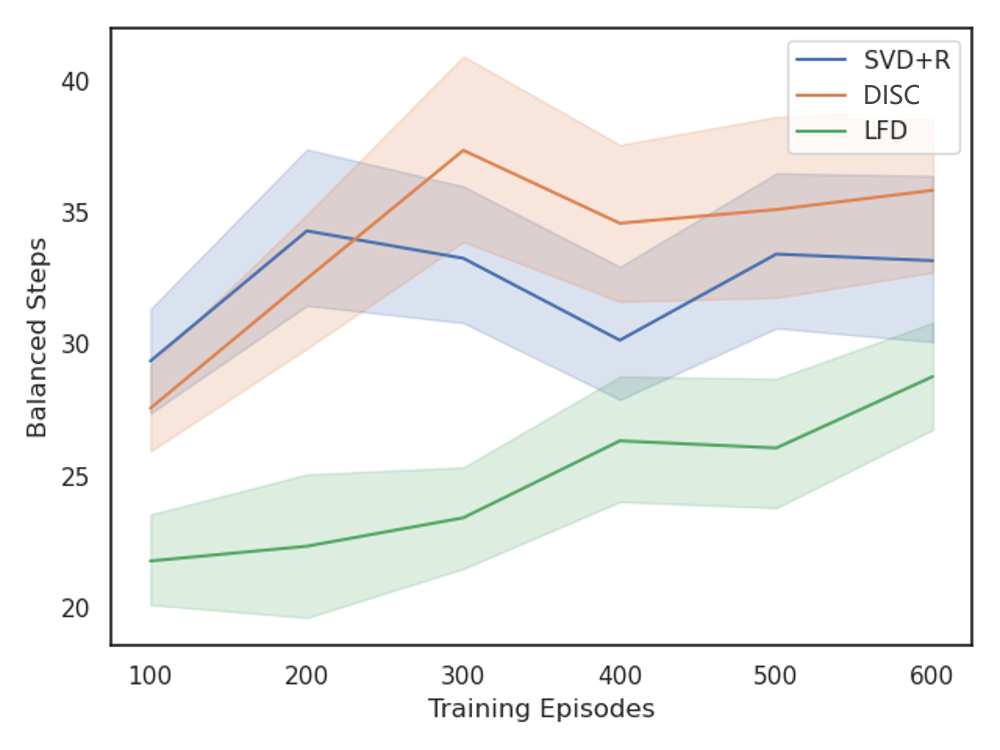
\includegraphics[scale=0.4]{BS.png}
    \caption{Average number of balancing steps with $k = 50$.}
    \label{fig: BS}
\end{figure}

\section{Conclusions and Future work}\label{sec:conclusion}
In this paper, we studied the problem of feature construction for linear value function approximation. Utilizing subspace invariance, we proposed DISCO algorithm based on orthogonal iteration method that ensures a theoretically tighter bound of Bellman error. Through the numerical results, we showed that our algorithm also outperforms other baseline methods empirically.

Although the linear value function approximation is less competitive than modern deep reinforcement learning, linear feature construction is still essential for nowadays network-based methods. Our future work aims to conjugate LVFA with current DRL methods, thus providing insights into the reinforcement learning problems.

\bibliographystyle{./bibliography/IEEEtran}
\bibliography{./bibliography/citation}

\end{document}
